\documentclass{article}
\usepackage{polyglossia}
\usepackage[a4paper]{geometry}
\usepackage{mathtools, amssymb, amsfonts}
\usepackage{amsthm}
\usepackage{fontspec}
\usepackage{titling}
\usepackage{listings}
\usepackage{graphicx}
\usepackage[hidelinks]{hyperref}
\usepackage{tikz}
\usepackage[locale = FR, inter-unit-product = .]{siunitx}
\usetikzlibrary{shapes,calc}
\usepackage[shortlabels]{enumitem}
\usepackage{comment}

\setdefaultlanguage{french}

%% Math commands
\renewcommand\epsilon\varepsilon
\renewcommand\phi\varphi
\newcommand{\N}{\mathbb N}
\newcommand{\Z}{\mathbb Z}
\newcommand{\R}{\mathbb R}
\newcommand{\Q}{\mathbb Q}
\newcommand{\CC}{\mathbb C}
\newcommand{\K}{\mathbb K}
\DeclarePairedDelimiter{\abs}{\lvert}{\rvert}
\DeclarePairedDelimiter{\norm}{\lVert}{\rVert}

%% Math environments
\theoremstyle{definition}
\newtheorem{exo}{Exercice}

%% Titling configuration
\pretitle{\begin{center}\LARGE}
\title{\textsc{Autour de l'Effet Doppler}}
\posttitle{\par\end{center}\vspace{-1.2em}}

\preauthor{}
\author{}
\postauthor{}

\date{\today}

\begin{document}
\maketitle

\begin{abstract}
	L'effet Doppler est le phénomène par lequel la perception d'un signal (acoustique, électromagnétique) émis par une source en mouvement relativement à un observateur présente, pour un signal monochromatique composé d'une seule fréquence, un décalage de celle-ci -- ou, pour un signal composé, un décalage de son spectre en fréquence.
\end{abstract}

\section{Introduction: le cas polychromatique}

On interprète souvent ce phénomène comme étant la perception d'une fréquence différente que celle émise par une source animée d'un mouvement. Le problème, c'est qu'avec des signaux quelconques, les notions de fréquence ou de longueur d'onde n'ont pas vraiment de sens : on peut parler de fréquence, à la rigueur, lorsque le signal est périodique, mais pour définir une longueur d'onde la signal doit être \textit{monochromatique} (par exemple, un son pur en acoustique). Comment donc décrire de façon pertinente l'effet Doppler quand on parle d'un signal quelconque qui serait néanmoins modifié par un déplacement de la source qui l'émet ?

\begin{figure}[!h]
	\centering
	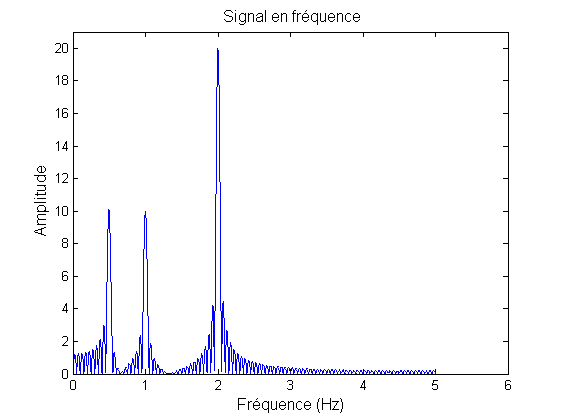
\includegraphics[width=0.6\textwidth]{fft.png}
	\caption{Un exemple de spectre en fréquence}
\end{figure}

On peut lever le problème en se ramenant au cas des signaux monochromatiques. Vous connaissez certainement le principe de la décomposition de Fourier: on peut écrire tout signal comme somme de signaux monochromatiques, de la forme $A(f)\cos(2\pi f t - \phi(f))$, où $A(f)$ est l'amplitude de l'harmonique de fréquence $f$ du signal initial et $\phi(f)$ sa phase. Vous avez mis en application ce principe en TP, lorsque vous avez réalisé à l'aide d'un logiciel les spectres en fréquence -- concrètement, les courbes de la fonction $A(f)$ -- de plusieurs signaux.

Pour cette raison, on peut simplifier le problème et se placer dans le cas où le signal émis est monochromatique: il est donc composé d'une seule longueur d'onde $\lambda$, à laquelle correspond une fréquence $f = c/\lambda$ où $c$ est la célérité des ondes dans le milieu.

\section{Démonstration de la formule de l'effet Doppler pour un signal de longueur d'onde $\lambda$}

Entre chaque émission d'un front d'onde s'écoule une durée égale à la période $T=\lambda/c=1/f$ de la source, celle-ci se déplace de $\vec v T$.

\begin{center}
	\begin{tikzpicture}
	\tikzset{dot/.style={circle,fill,inner sep=2pt}}
	\node (S) at (0,0) [dot, label={260:Source $S$}]{};
	\draw [blue, ->,thick] (S) -- node[label={[black]90:$\vec v$}] {} (1,0.5) -- (2,1);
	
	\foreach \r in {0.7,1.4,2.1,2.8}
	\draw (-0.5*\r,-0.25*\r) circle (\r) [red, dashed, thick];
	
	\node (M) at (4,0) [dot,label={$P$}]{};
	\draw[->,thick] (S) -- node[label={-25:$\vec u$}]{} ++(2,0);
	\end{tikzpicture}
\end{center}

Si le vecteur \textbf{unitaire} $\vec u$ représente la ligne de visée de l'observateur, la distance entre les fronts d'ondes émis entre $t$ et $t+T$ est 
\begin{equation}\boxed{
\lambda' = \lambda - (\vec vT)\cdot\vec u =  (c-\vec v\cdot\vec u)T.}
\end{equation}

En effet, la distance entre deux fronts est la longueur d'onde initiale $\lambda = cT$, amputée du déplacement de la source dans la direction de l'observateur (puisque ce déplacement fait que la nouvelle émission sera effectuée plus proche de celui-ci), c'est à dire $\vec v T \cdot \vec u = (\vec v \cdot \vec u)T$.

\begin{center}
	\begin{tikzpicture}
	\tikzset{dot/.style={circle,fill,inner sep=1.5pt}}
	\node[dot, label={180:$S(t)$}](S1) at (0,0) {};
	\node[dot, label=$S(t+T)$](S2) at (1.5,2) {};
	\node[dot, label=$P$](P) at (3,0) {};
	
	\draw[->,blue,thick] (S1)-- (0.75,1) node[label={180:$\vec vT$}]{} --(S2);
	\draw[-,red,dashed] (S1)--(P);
	\draw[->,thick] (S1)-- (0.5,0) node[label={30:$\vec{u}$}] {};
	
	\draw[dotted] (S2)--(1.5,0) node[dot,inner sep=1pt](pS2){};
	\draw[<->,gray] (0,-0.2) -- (.75,-0.2) node[label={[black]270:$(\vec vT)\cdot \vec u$}]{} -- (1.5,-0.2);
	\end{tikzpicture}
\end{center}

La fréquence du signal perçu est alors
\begin{equation}
	f' = \frac{c}{\tilde{\lambda}} = \frac{c}{(c-\vec v \cdot \vec u)T}\quad\text{soit}\quad
	\boxed{f' = \frac{c}{c-\vec v\cdot\vec u}f.}
\end{equation}

\begin{exo}
	Démontrer la formule approchée
	\begin{equation}
		f' \simeq \left(1+\frac{\vec v\cdot \vec u}{c}\right)f
	\end{equation}
	pour $\norm{\vec v}\ll c$.
	
	On donne que pour $x\ll 1$, $\dfrac{1}{1-x}\simeq 1+x$.
\end{exo}

\begin{exo}
	On considère un véhicule de police traversant une intersection dont les rues sont à un angle de 30 degrés, à une vitesse de \SI{70}{\kilo\meter\per\hour}.
	 	
	Un microphone dans l'habitacle du véhicule enregistre le son émis par la sirène à une fréquence d'échantillonnage de \SI{2048}{\hertz}. Le signal reconstitué, ainsi que son spectre en fréquence sont fournis ci-dessous.
	
	\begin{figure}[h]
		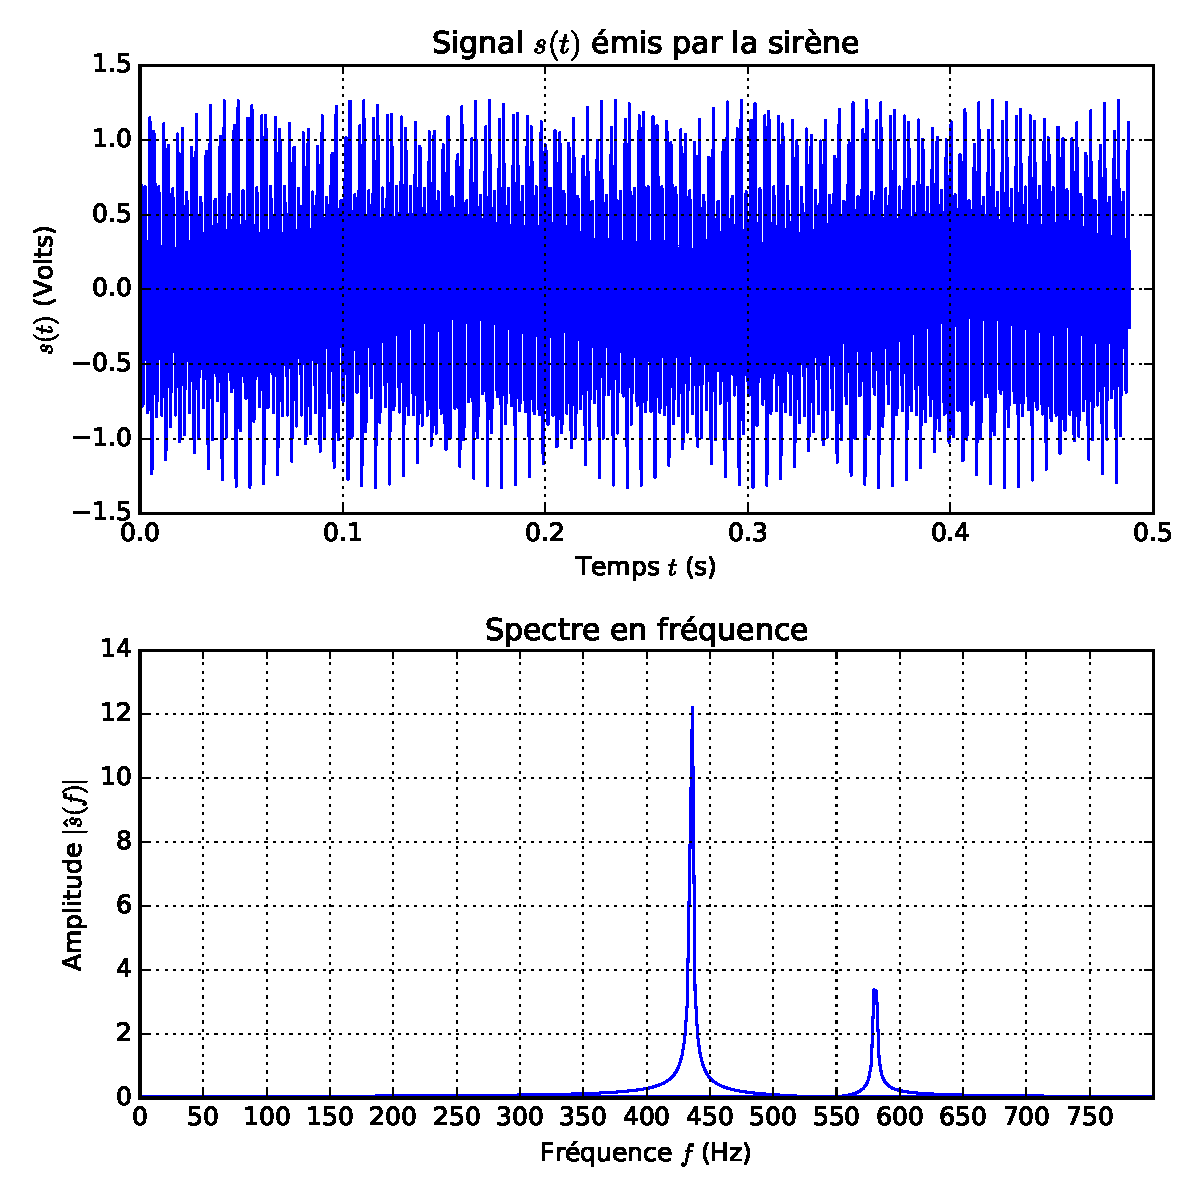
\includegraphics[width=\textwidth]{python-scripts/sirene.pdf}
	\end{figure}
	
	Un observateur se situe dans la rue croisant celle traversée par le véhicule. Quelles sont les fréquences principales du son qu'il entend quand la voiture passe juste devant lui ? Dessiner son spectre de Fourier. Proposer une expression du signal $s_\mathrm{reçu}(t)$ correspondant.
\end{exo}

\section{Effet Doppler-Fizeau}

L'effet Doppler se généralise à toute situation mettant en jeu des ondes, y compris en dehors de l'acoustique. Dans le domaine des ondes électromagnétiques, on observe un effet Doppler lumineux : la lumière reçue par un observateur provenant d'une source lumineuse en mouvement change de couleur. Ou, du moins, on peut observer un décalage dans le spectre de la lumière reçue par rapport à un spectre d'émission (ou d'absorption...) de référence.

En astronomie, on l'utilise pour évaluer, à partir de ce décalage, la vitesse à laquelle se déplace des sources de lumière (astres, galaxies...) très éloignées de nous. On peut également détecter le mouvement de nébuleuses en cherchant un déplacement des raies d'absorption caractérisant les éléments présents dans les poussières qui les constituent.

Lorsque le décalage en fréquence se fait vers le domaine du bleu, on parle de \textit{blue shift}; vers le rouge, on parle de \textit{red shift}.

\begin{figure}[h]
	\centering
	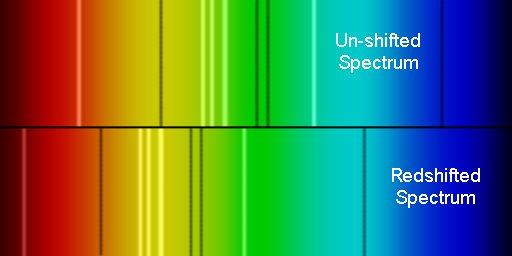
\includegraphics[width=0.8\textwidth]{redshift1.jpg}
	\caption{Spectre d'absorption d'un corps au repos, et spectre \textit{redshifté} lors du mouvement de celui-ci.}
\end{figure}

Dans le cas où la source est à une vitesse \textit{non-relativiste}, c'est-à-dire $v\ll c$, les formules précédentes sont toujours valables (sinon, il faut corriger en utilisant la théorie de la relativité restreinte... bref.)

\begin{exo}
	Les \textit{raies de Balmer} sont les raies du spectre d'émission de l'hydrogène qui correspondent aux transitions énergétiques vers l'état d'énergie $n=2$. La première raie, notée H$\alpha$, correspondant à la transition énergétique $3\to 2$, a pour longueur d'onde $\lambda = \SI{656.3}{\nano\meter}$.
	
	\begin{enumerate}
		\item Quelle est sa couleur ?
		\item On considère un corps contenant de l'hydrogène. Une étude du spectre lumineux reçu montre un décalage de la série des raies de Balmer plaçant H$\alpha$ une longueur d'onde de $\SI{682.1}{\nano\meter} $. L'objet se rapproche-t-il ou s'éloigne-t-il ? Quelle est sa vitesse ? Sommes-nous toujours dans un cadre non-relativiste ?
	\end{enumerate}
\end{exo}

\end{document}